\section{Αθροιστής υπολοίπου $2^n-1$}
\label{section:mod_addition}
Η αριθμητική υπολοίπου αφορά το υπόλοιπο ενός αριθμού X διαιρεμένου με έναν Y, εναλλακτικά
αφαιρείτε από το Χ το Y μέχρι $X < Y$. Η πράξη αυτή συμβολίζεται ως 
\begin{equation*}
    X\ mod\ Y
\end{equation*}
Αριθμητικές υπολοίπου είναι χρήσιμες σε ένα μεγάλο πλήθος εφαρμογών εφόσον αποτελούν και 
την βάση για τα Residue Number Systems (RNS). Επίσης αποτελούν μέρος της ψηφιακής
επεξεργασίας σημάτων και ψηφιακών φίλτρων, κρυπτογραφίας, σε τεχνικές ανίχνευσης και διόρθωσης σφάλματος καθώς και σε υψηλών ταχυτήτων δίκτυα. Η δυαδική άθροιση εκφράζεται μέσω αριθμητική υπολοίπου ως $(A+B)\ mod\ n$, όπου n είναι το πλήθος των δυαδικών ψηφίων των A και B. Στην παρούσα ενότητα θα μελετηθούν οι αθροιστές υπολοίπου $2^n-1$ όπου η επιτάχυνση τους είναι ο σκοπός του παρόν έργου.






\subsection{Μαθηματική προσέγγιση}
Ο μαθηματικός υπολογισμός του αθροίσματος υπολοίπου $2^n-1$ στην πραγματικότητα είναι 
ένας υπο-συνθήκη υπολογισμός με συνθήκη $A+B < 2^n$ και ορίζεται ως 
\begin{equation}
\label{eq:Modulo_2^n-1}
\equationame{Ορισμός άθροισης υπολοίπου $2^n-1$}
(A+B)\, mod\, (2^n-1) = 
\begin{cases}
    (A+B)\, mod\; 2^n       , &  A+B < 2^n\\
    (A+B)\, mod\; 2^n + 1   , & A+B \geq 2^n
\end{cases}
\end{equation}
Ο ορισμός αυτός μαθηματικά έχει ένα λάθος, το οποίο όμως λαμβάνοντας μία 
παραδοχή, θα εξαλειφθεί.
Για παράδειγμα, έστω πως $n=3$ άρα και $2^n-1 = 7$, όπου n το πλήθος των δυαδικών ψηφίων
που έχει κάθε αριθμός εισόδου. Για τον υπολογισμό του υπολοίπου, όπως προαναφέρθηκε,
διαιρείται ο αριθμός εισόδου με το 7 και το υπόλοιπο είναι το αποτέλεσμα. Με είσοδο 
τον αριθμό 3 υπολογίζεται $3/7 = 0$ και υπόλοιπο 3. Παρακάτω παρουσιάζεται μια σειρά από 
παραδείγματα.
\begin{equation*}
    \begin{split}
        8\ mod\ 7 &= 1 \\
        7\ mod\ 7 &= 0 \\
        14\ mod\ 7 &= 0 \\
        6\ mod\ 7 &= 6 \\
        13\ mod\ 7 &= 6
    \end{split}
\end{equation*}
Όπως είναι εμφανές και στα παραδείγματα ο μαθηματικός υπολογισμός που ορίστηκε φαίνεται να 
μην ισχύει για την περίπτωση $7\ mod\ 7$ διότι ο αριθμός 7 είναι μικρότερος του $2^n = 2^3 = 8$,
άρα ανήκει στην πρώτη περίπτωση της εξίσωσης \ref{eq:Modulo_2^n-1} όπου σύμφωνα με αυτή το 
αποτέλεσμα θα έπρεπε να ήταν επτά και όχι μηδέν. Σε αυτό το σημείο λοιπόν είναι σημαντικό
να τονιστεί πως χρησιμοποιείται διπλή αναπαράσταση του μηδέν. Η μία αναπαράσταση είναι η 
προφανής όπου όλα τα ψηφία είναι 0 και η δεύτερη είναι η $2^n-1$, δηλαδή όλα τα ψηφία 
να είναι στο 1. Αυτό το φαινόμενο δεν είναι πάντα επιθυμητό. Στην συνέχεια του κεφαλαίου
θα δοθεί μια πρόταση για την αντιμετώπιση της διπλής αυτής αναπαράστασης.

Υπάρχουν διάφοροι τρόποι για να υπολογιστεί στο υλικό το αποτέλεσμα 
ενός αθροιστή υπολοίπου $2^n-1$.
Η πιο απλή ιδέα αποτελείται από δύο αθροιστές όπου ο πρώτος δεν έχει
κρατούμενο εισόδου, παίρνει ως είσοδο τα Α και Β και η έξοδος του τροφοδοτεί
την είσοδο του δεύτερου αθροιστή με δεύτερο όρισμα τον μηδενικό αριθμό
και κρατούμενο εισόδου το κρατούμενο εξόδου του πρώτου αθροιστή. Το άθροισμα 
του δεύτερου αθροιστή είναι και το ζητούμενο. Στην εικόνα \ref{fig:2^n-1_simple_adder}
αποτυπώνεται η απλή αρχιτεκτονική που περιγράφηκε.
\begin{figure}[H]
    \centering
    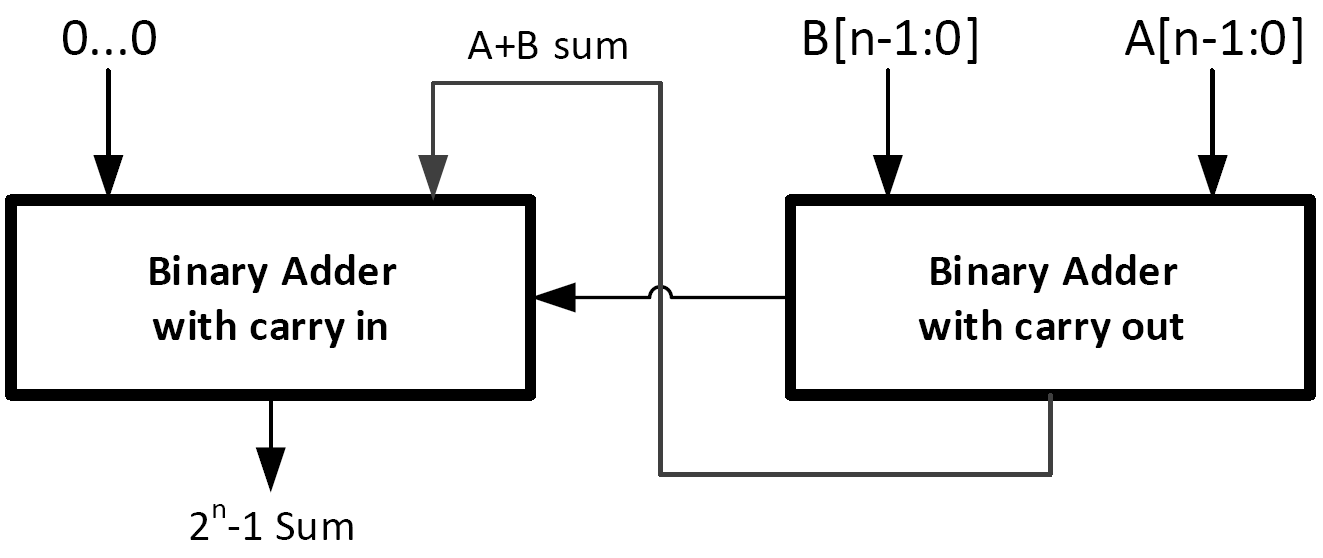
\includegraphics[height=4cm,width=9cm]{Simple_2^n-1_adder.png}
    \caption{Απλή δομή αθροιστή υπολοίπου $2^n-1$}
    \label{fig:2^n-1_simple_adder}
\end{figure}
Η παραπάνω τεχνική έχει πολύ μεγάλη χρονική καθυστέρηση διότι υπάρχουν δύο 
επίπεδα αθροιστών. Για να μειωθεί ο χρόνος που απαιτείται για να οδηγηθεί η έξοδος
με το σωστό αποτέλεσμα είναι δυνατή η παράλληλη εκτέλεση δυο προθέσεων του Α και Β
με τον ένα αθροιστή να έχει κρατούμενο εισόδου και τον άλλο χωρίς. Τα αποτελέσματα 
των δύο αθροιστών θα οδηγούνται σε έναν πολυπλέκτη με είσοδο επιλογής το κρατούμενο 
εξόδου του αθροιστή χωρίς κρατούμενο εισόδου. Αν η είσοδος επιλογής είναι ενεργή 
τότε θα επιλέγεται η έξοδος του αθροιστή με κρατούμενο εισόδου όπως φαίνεται στην 
 εικόνα \ref{fig:2^n-1_carry_select_adder}.
\begin{figure}[H]
    \centering
    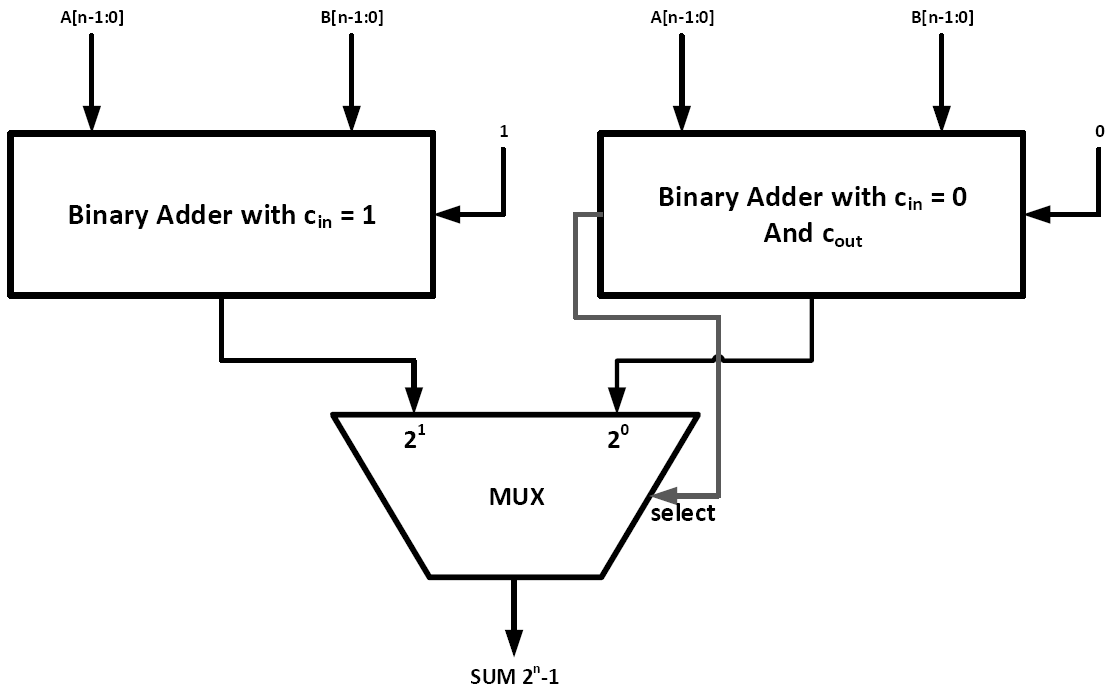
\includegraphics[height=4cm,width=8.5cm]{Carry_select_2^n-1.png}
    \caption{Αρχιτεκτονική αθροιστή επιλογής κρατουμένου $2^n-1$}
    \label{fig:2^n-1_carry_select_adder}
\end{figure}
Πρέπει να σημειωθεί πως και στις δύο περιπτώσεις απαιτείται η υλοποίηση δύο αθροιστών 
με αποτέλεσμα να αυξάνεται το εμβαδόν του αθροιστή στο διπλάσιο συγκριτικά με έναν απλό αθροιστή.
Ένας ακόμα παράγοντας σε αυτές τις αρχιτεκτονικές είναι η δομή των επιμέρους αθροιστών. 
Η επίτευξη υψηλών ταχυτήτων είναι δυνατή επιλέγοντας μια παράλληλη προθεματική δομή 
για τον σχεδιασμό των αθροιστών που συντελούν τον αθροιστή υπολοίπου, θυσιάζοντας αρκετά
τον χώρο και την κατανάλωση.

Μία καθιερωμένη υλοποίηση των αθροιστών αυτής της κατηγορίας χρησιμοποιεί έναν τυπικό αθροιστή
συνδέοντας το κρατούμενο εξόδου στο κρατούμενο εισόδου δημιουργώντας έναν αθροιστή κυκλικού
κρατουμένου (end-round carry). Αυτή η τοπολογία μετατρέπει τον αθροιστή σε ένα ασύγχρονο 
ακολουθιακό κύκλωμα, του οποίου η κατάσταση εξαρτάται από προηγούμενες καταστάσεις και από την 
καθυστέρηση της διάδοσης κρατουμένων. Εξαιτίας αυτής της συμπεριφοράς δημιουργούνται
πρακτικά προβλήματα χρονισμού με αποτέλεσμα την επιπλέον αύξηση του χρόνου καθυστέρησης.
Το πρόβλημα αυτό παρατηρείται στις περιπτώσεις που οι δυαδικοί αριθμοί εισόδου 
είναι συμπληρωματικοί ως προς ένα και αντιμετωπίζεται οδηγώντας την είσοδο 
κρατουμένου με την παρακάτω συνάρτηση και όχι απευθείας με το κρατούμενο εξόδου \cite{1674817}.
\begin{equation}
    C_{in} = C_{out} + P_{n-1:0}
\end{equation}
Με αυτήν την μικρή διαμόρφωση αντιμετωπίζεται επίσης και η διπλή αναπαράσταση του μηδέν.
Η μόνη περίπτωση που προκύπτει η δεύτερη αναπαράσταση του μηδέν ($1...11$) πετυχαίνεται
όταν οι αριθμοί εισόδου είναι συμπληρωματικοί. Με την παραπάνω τροποποίηση όμως στην περίπτωση αυτή το σήμα $P_{n-1:0}$ ενεργοποιείται και οδηγεί το κρατούμενο εισόδου, 
με προφανές τελικό αποτέλεσμα το μηδέν στην κανονική αναπαράστασή του.

Στην συνέχεια της εργασίας αυτής οι αθροιστές υπολοίπου που θα παρουσιαστούν ή θα 
σχεδιαστούν, θα είναι με την σύμβαση της διπλής αναπαράστασης. Συγκριτικά, οι αθροιστές
με διπλή αναπαράσταση είναι ταχύτεροι και απαιτούν λιγότερους πόρους από αυτούς
με μονή αναπαράσταση \cite{298378}. Αυτός είναι και ο λόγος που οι αυτοί αθροιστές  
προτιμούνται στις περιπτώσεις που είναι εφικτοί. Αν η εφαρμογή απαιτεί μονή αναπαράσταση 
τότε η πρόσθεση επιπλέον λογικής στους αθροιστές είναι αναπόφευκτη.

















\subsection{Prefix αθροιστές $2^n-1$ }
% -----------------------------------------------
% G_{} = τα κρατούμενα του πρώτου επιπέδου 
% G_{}^' = τα κρατούμενα του δεύτερου επιπέδου
% -----------------------------------------------
Εξετάζεται η περίπτωση ενός αθροιστή που αποτελείται από δύο στάδια, το πρώτο χωρίς κρατούμενο εισόδου
και το δεύτερο στάδιο έχει κρατούμενο εισόδου το κρατούμενο εξόδου του πρώτου. Οπότε στο
πρώτο στάδιο $c_{-1} = 0$. Από την εξίσωση \ref{eq:G'P'_From_GP} συμπεραίνετε πως 
$(G'_{n-1},P'_{n-1}) = (G_{n-1},P_{n-1})$. Στο δεύτερο επίπεδο ισχύει 
$c_{-1} = G'_{n-1} = G_{n-1} $ εφόσον στο πρώτο στάδιο το κρατούμενο εισόδου είναι μηδέν.
Για $c_{-1} = G_{n-1}$ η εξίσωση \ref{eq:G'P'_From_GP} παίρνει την μορφή 
\begin{equation*}
\begin{split}
    (G'_{n-1},P'_{n-1}) &= ( G_{n-1} + P_{n-1}*c_{-1} ,  P_{n-1} )\\
    &=( G_{n-1} + P_{n-1}*G_{n-1} ,  P_{n-1} )\\
    &=(G_{n-1},P_{n-1})
\end{split}    
\end{equation*}
Αποτέλεσμα της παραπάνω εξίσωσης είναι πως το κρατούμενο εξόδου του δεύτερου επίπεδου 
$c'_{n-1} = G'_{n-1}$
( αν και δεν αφορά άμεσα την υλοποίηση εφόσον δεν υπάρχει λόγος υπολογισμού του 
στους αθροιστές υπολοίπου $2^n-1$) είναι σταθερό από το πρώτο επίπεδο και παραμένει και στο 
δεύτερο. Επίσης από την εξίσωση \ref{eq:G'P'_From_GP} ισχύει 
\begin{equation}
\label{eq:2^n-1_G'_eguation}
    (G'_i,P'_i) = (G_i + P_iG_{n-1} , P_{i})
\end{equation}

\begin{figure}[H]
    \centering
    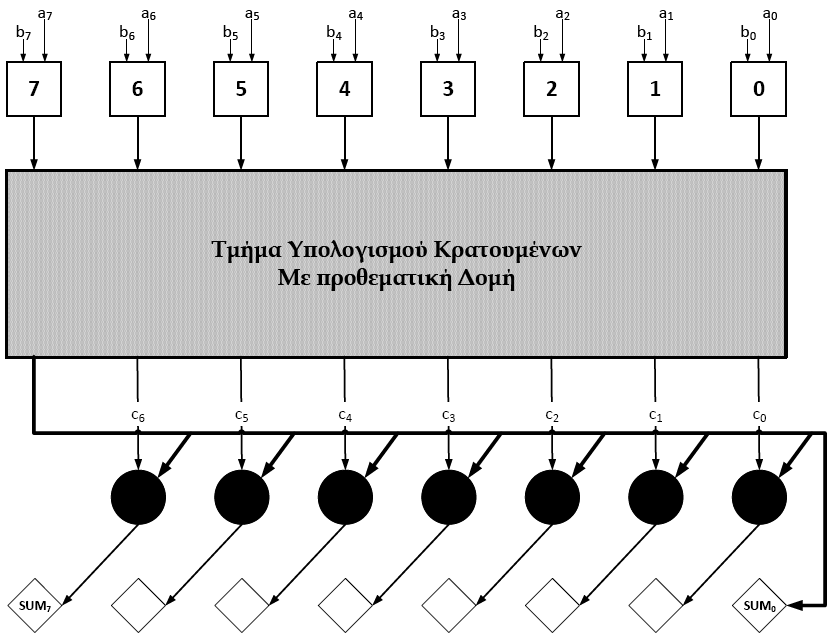
\includegraphics[width=height=6cm,width=9cm]{2^n-1_simple_Prefix_structure.png}
    \caption{Απλή δομή προθεματικού αθροιστή υπολοίπου $2^8-1$}
    \label{fig:2^n-1_simple_Prefix_structure}
\end{figure}
Στην εικόνα \ref{fig:2^n-1_simple_Prefix_structure} παρουσιάζεται η βασική δομή των αθροιστών υπολοίπου υλοποιημένη με προθεματικό αθροιστή σύμφωνα με τις εξισώσεις που αναπτύχθηκαν.
Ένας σχεδιασμός σαν τον παραπάνω, εκτός από το γεγονός του επιπλέον επιπέδου,
έχει και το μειονέκτημα στο ότι το κρατούμενο εξόδου του πρώτου τμήματος οδηγεί 
n κόμβους του τελευταίου επιπέδου, όπως εκφράζεται και από την εξίσωση \ref{eq:2^n-1_G'_eguation}.

















\subsection{Αρχιτεκτονική βελτιστοποίηση}

Χρησιμοποιώντας τον ειδικό τελεστή που παρουσιάστηκε στο κεφάλαιο 4 $"\circledast"$
ο αθροιστής υπολοίπου $2^n-1$ μπορεί να υλοποιηθεί με ένα ακόμα παράλληλο τμήμα 
με αποτέλεσμα να μειωθεί κατά ένα επίπεδο ο υπολογισμός του \cite{863036}.
% -----------------------------------------------
% G_{} = τα κρατούμενα του πρώτου επιπέδου 
% G_{}^' = τα κρατούμενα του δεύτερου επιπέδου
% G_{}^* = τα κρατούμενα της νέας αρχιτεκτονικής
% -----------------------------------------------
Όπως εξηγήθηκε προηγουμένως το κρατούμενο εισόδου, στο δεύτερο επίπεδο, του αθροιστή υπολοίπου n
δυαδικών ψηφίων είναι ίσο με το κρατούμενο εξόδου του στο πρώτο επίπεδο, που είναι 
χωρίς κρατούμενο εισόδου, $c_{-1} = G_{n-1}$, άρα ισχύει και 
$(G^*_{-1},P^*_{-1}) = (G_{n-1},P_{n-1})$, συμβολίζοντας $G^*$ τα κρατούμενα που υπολογίζονται 
στο δεύτερο επίπεδο.\\\\
% Proof
% -----------------------------------------------
Με επαγωγικό τρόπο θα αποδειχθεί πως
\begin{equation}
\label{eq:(G*,P*)}
\equationame{Εξίσωση κρατουμένων του $2^n-1$ αθροιστή}
    (G^*_i,P^*_i) =
    \begin{cases}
        (G_{n-1},P_{n-1}) ,& i = -1\\
        (g_i,p_i)\circledast(G^*_{i-1},P^*_{i-1}) ,& 0\leq i \leq n-2
    \end{cases}
\end{equation}
Απόδειξη :
\begin{enumerate}
    \item Για $i=-1$ ισχύει $(G^*_{-1},P^*_{-1}) = (G_{n-1},P_{n-1})$. Όπως προαναφέρθηκε προηγουμένως, $c_{-1} = G_{n-1}$ , $c^*_{-1} = G^*_{-1}$. Άρα $c^*_{-1} = G^*_{-1}$.
    \item Αρχική υπόθεση πως η εξίσωση \ref{eq:(G*,P*)} ισχύει και για $i=k-1$ με $k \geq 0$.
    Άρα ισχύει και $c^*_{k-1} = G^*_{k-1}$. Θα αποδειχθεί πως ισχύει και για $i=k$. Ξεκινώντας 
    με τον ορισμό και έχοντας την παραπάνω υπόθεση αποδεικνύεται 
    \begin{equation*}
    \begin{split}
        (G^*_k,P^*_k) &= (g_k,p_k) \circledast (G^*_{k-1},P^*_{k-1})\\
        &= (g_k,p_k) \circledast (c^*_{k-1},P^*_{k-1})\\
        &= (g_k + p_k c^*_{k-1} , p_k P^*_{k-1})\\
        &= (c^*_{k},P_k)
    \end{split}
    \end{equation*}
    Σύμφωνα με τις παραπάνω ισότητες, ισχύει $c^*_i = G^*_i$ για $-1 \leq i \leq n-2$.
\end{enumerate}

Πριν την παρουσίαση της νέας δομής, η οποία έχει ένα λιγότερο επίπεδο από την δομή 
που περιγράφηκε παραπάνω, πρέπει να γίνει μία απόδειξη ενός ισχυρισμού που θα χρειαστεί στην 
συνέχεια. Ο ισχυρισμός αυτός είναι
\begin{equation}
\label{eq:GgG=Gg}
    (G_i,P_i)\circledast(g,p)\circledast(G_i,P_i) = (G_i,P_i)\circledast(g,p)
\end{equation}
Απόδειξη
\begin{equation*}
    \begin{split}
        (G_i,P_i)\circledast(g,p)\circledast(G_i,P_i) &= (G_i + P_i*g,P_i*p) \circledast (G_i,P_i) \\
        &= (G_i + P_i*g + P_i*p*G_i , P_i*p*P_i)\\
        &= (G_i*(1 + P_i*p) + P_i*g , P_i*p )\\
        &= (G_i + P_i*g , P_i * p)\\
        &= (G_i,P_i) \circledast (g,p)
    \end{split}
\end{equation*}
\\
Από την εξίσωση \ref{eq:(G*,P*)} αποδεικνύεται 
\begin{equation}
\label{eq:(G*,P*)_new}
    \begin{split}
        (G^*_i,P^*_i) &= (g_i,p_i) \circledast (G^*_{i-1},P^*_{i-1})\\
        &= (g_i,p_i) \circledast (g_{i-1},p_{i-1}) \circledast ... \circledast (g_0,p_0) \circledast (G^*_{-1},P^*_{-1})\\
        &= (g_i,p_i) \circledast ... \circledast (g_0,p_0) \circledast (G_{n-1},P_{n-1})\\
        &= (g_i,p_i) \circledast ... \circledast (g_0,p_0) \circledast (g_{n-1},p_{n-1}) \circledast (G_{n-2},P_{n-2})\\
        &= (g_i,p_i) \circledast ... \circledast (g_0,p_0) \circledast (g_{n-1},p_{n-1})
        \circledast ... \circledast (g_i,p_i) \circledast ... \circledast (g_0,p_0)\\
        &= (G_i,P_i) \circledast (g_{n-1},p_{n-1}) \circledast ... \circledast (g_{i+1},p_{i+1})
        \circledast (G_i,P_i)\\
        (G^*_i,P^*_i) &= (G_i,P_i) \circledast (g_{n-1},p_{n-1}) \circledast ... \circledast (g_{i+1},p_{i+1})
    \end{split}
\end{equation}
Στην τελευταία ισότητα της παραπάνω διαδικασίας εφαρμόζεται ο ισχυρισμός της εξίσωσης \ref{eq:GgG=Gg}.
Η σχέση της εξίσωσης \ref{eq:(G*,P*)_new} είναι και η αρχιτεκτονική βελτίωση των αθροιστών υπολοίπου
$2^n-1$.

Σε αυτό το σημείο είναι αναγκαίο να δηλωθεί μια αναπαράσταση με σκοπό την ευκολία στην
έκφραση συναρτήσεων και όρων. Το σήμα $G_{i}$ αντιπροσωπεύει το $G_{i:0}$, δηλαδή
έχει κάθε ζευγάρι $(g_k,p_k)$, με $ i \geq k \geq 0 $, με τον τελεστή $\circledast$.
Είναι δυνατό, όπως έχει προαναφερθεί, να έχουμε τον όρο $G_{i:j}$, με $ i \geq j$ με
την περίπτωση της ισότητας τότε το $G_{i:i} = g_i$ και στην περίπτωση όπου το $j=0$ ισχύει $G_{i:0}=c_i$. Θα οριστεί μια νέα έκφραση, η οποία 
προβλέπει την περίπτωση του $i < j$ στην έκφραση $G_{i:j}$. Διατυπώνεται λοιπόν ο παρακάτω συμβολισμός.
% \begin{equation*}
%     (G_{i:j},P_{i:j} = (G_i,P_i) \circledast (G_{n-1:j},P_{n-1:j})
% \end{equation*}

\begin{equation}
    (G_{i:j},P_{i:j}) =
    \begin{cases}
        (g_i,p_i)\circledast(g_{i-1},p_{i-1})\circledast...\circledast(g_j,p_j) ,& i > j \\
        (g_i,p_i) ,& i = j \\
        (G_{i:0},P_{i:0}) \circledast (G_{n-1:j},P_{n-1:j}) ,& i < j
    \end{cases}
\end{equation}
όπου n είναι το μέγεθος του αθροιστή. Έχοντας ορίσει την παραπάνω έκφραση, είναι αποδεκτή και μια εναλλακτική διατύπωση των σημάτων $(G^*_i,P^*_i)$
\begin{equation}
    (G^*_i,P^*_i) = (G_{i:i+1},P_{i:i+1})
\end{equation}
Το ίδιο ισχύει και για τους υπόλοιπους όρους (P,H,Q).
Για παράδειγμα σε ένα αθροιστή των οκτώ δυαδικών ψηφίων $n=8$, για τον υπολογισμό του 
$G_{1:6}$ υπονοείται η παρακάτω έκφραση :
\begin{equation*}
    G_{1:6} = g_1 + p_1g_0 + p_1p_0g_7 + p_1p_0p_7g_6
\end{equation*}
Είναι σημαντικό να ξεκαθαριστεί πως αυτός ο τρόπος διατύπωσης είναι χρήσιμος στην περιγραφή μόνο αθροιστών υπολοίπου $2^n-1$. Στις περιπτώσεις άλλων αθροιστών καθίσταται απαγορευμένη έκφραση. Στην παρακάτω εικόνα εφαρμόζεται η διαδικασία αυτή για το $G_{4:5} = G^*_{4}$. Είναι εμφανές πως το προηγούμενο στοιχείο του μηδέν είναι το $n-1$, δηλαδή το επτά στην περίπτωση του $2^8-1$ αθροιστή υπολοίπου των 8-bits. 
\begin{figure}[H]
    \centering
    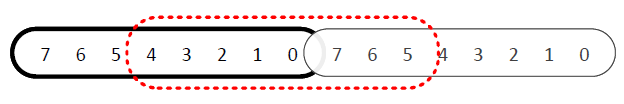
\includegraphics[scale=0.6]{Round_numbers.png}
    % \caption{}
    % \label{}
\end{figure}


Στην εικόνα \ref{fig:2^8-1_new_structure} παρουσιάζεται η αρχιτεκτονική ενός 8-bit αθροιστή υπολοίπου $2^n-1$ με σκοπό την οπτικοποίηση της παραπάνω κυκλικής έκφρασης. Συγκρίνοντας αυτή την τοπολογία με αυτή της εικόνας \ref{fig:2^n-1_simple_Prefix_structure}, είναι εμφανές η διαφορά του επιπλέον επιπέδου.
\begin{figure}[H]
\centering
% 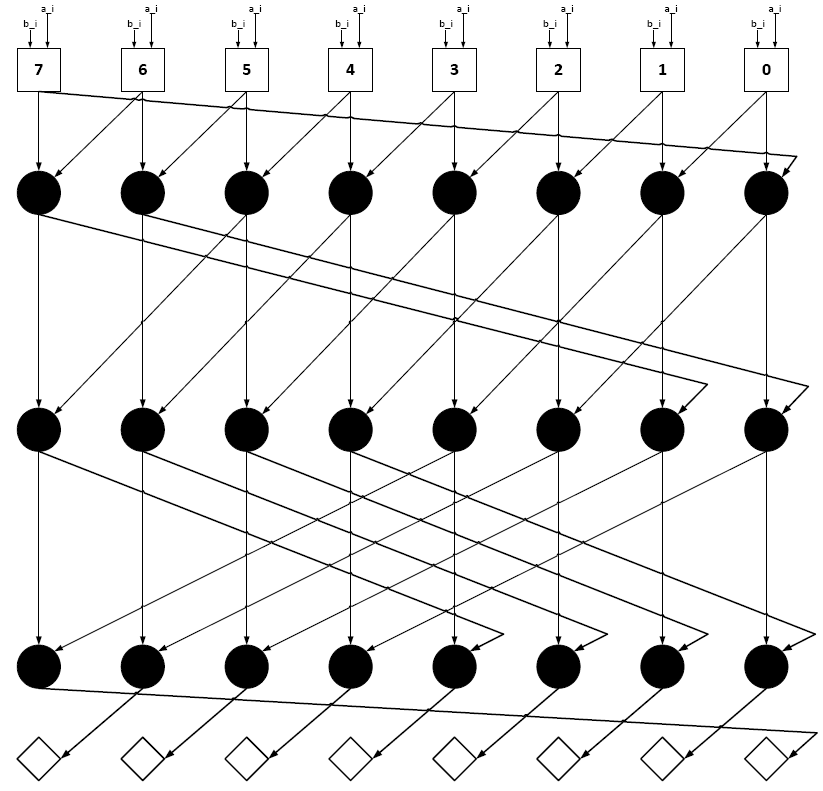
\includegraphics[width=\textwidth]{2^8-1_new_structure.png}
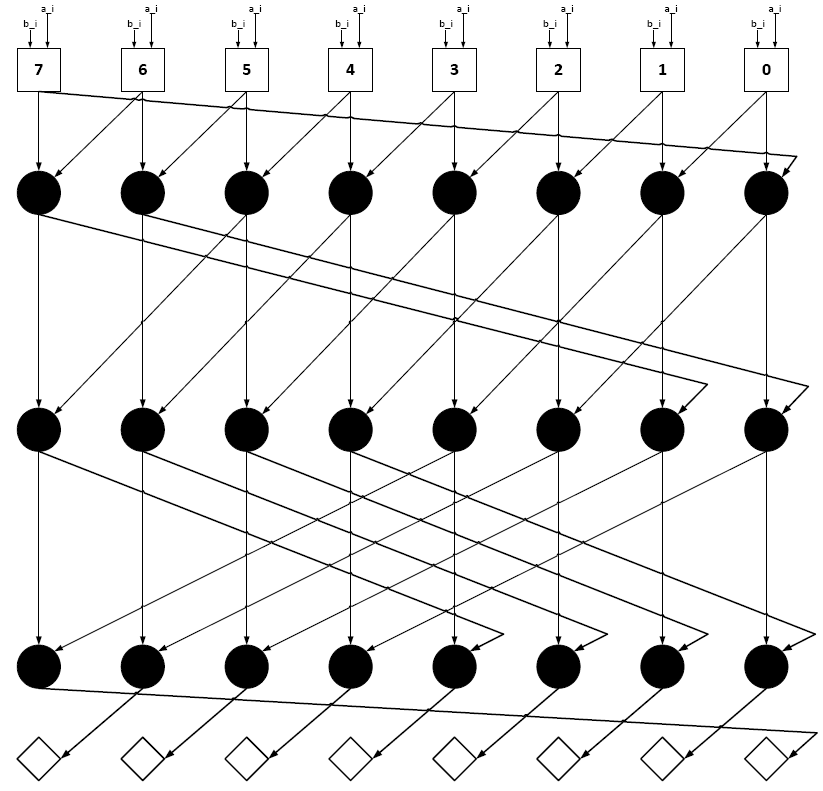
\includegraphics[width=height=6cm,width=9cm]{2^8-1_new_structure.png}
\caption{Παράλληλος προθεματικός αθροιστής υπολοίπου $2^8-1$}
\label{fig:2^8-1_new_structure}
\end{figure}





